\documentclass[a4paper, DIV11, abstracton]{scrartcl}
\usepackage{color,graphicx}			% graphics package

\usepackage{microtype}				% optical margin alignment
\usepackage[T1]{fontenc}			% umlauts for european languages
\usepackage{textcomp}				% provides extra symbols
\usepackage[utf8]{inputenc}			% character encoding
\usepackage[USenglish]{babel}		% elements language and hyphenation

\usepackage[round]{natbib}			% scientific bibliography
%\usepackage{url}					% nicely spaced urls
\usepackage{amsmath}				% mathematical equation alignment
%\usepackage{dcolumn}				% decimal alignment in tables
\usepackage{siunitx}				% units (micrometers, anyone?)
\usepackage[font=small, format=plain, labelsep=period, labelfont={sf,bf}, justification=justified]{caption}	% formatting the labels for figures, tables

% fonts
\usepackage{palatino}
\usepackage{mathpazo}
\usepackage[scaled=0.92]{helvet}

\setcounter{secnumdepth}{1}			% only number top headings (\section)
\setcounter{tocdepth}{2}			% include \subsection in TOC

\usepackage[raiselinks, pdfborder={0 0 0}]{hyperref}  % creates pdf sections for acrobat
%\hypersetup{pdftitle={Title}}




\begin{document}


\title{Matlab 2011}
\author{Christoph Rieper and Benjamin Sunarjo}


\maketitle
%\thispagestyle{empty} % no page numbers on title page

Document Version: 1.0\\*
Group Name: Rieparjo\\*
Group Members: Christoph Rieper and Benjamin Sunarjo


\setcounter{page}{1}	% start page numbering here
%=-=-=-=-=-=-=-=-=-=-=-=-=-=-=-=-=-=-=-=-=-=-=-=-=-=-=-=-=-=-=-=-=-=
\section{Introduction}
%=-=-=-=-=-=-=-=-=-=-=-=-=-=-=-=-=-=-=-=-=-=-=-=-=-=-=-=-=-=-=-=-=-=

%(States your motivation clearly: why is it important / interesting to solve this problem?)
%(Add real-world examples, if any)
%(Put the problem into a historical context, from what does it originate? Are there already some proposed solutions?)

Agent-based models can provide a easily implementable way to study complex systems. As \citet{helbing:1997} have shown, many aspects of pedestrian motion, such as the formation of trail systems in green areas, can be reproduced using a relatively simple ``active walker'' model that takes into account the attractiveness of terrain and feedback on the terrain as it is walked upon. In the current project, we plan to apply such an active walker model to real landscapes and compare the results to existing road systems.



%=-=-=-=-=-=-=-=-=-=-=-=-=-=-=-=-=-=-=-=-=-=-=-=-=-=-=-=-=-=-=-=-=-=
\section{Fundamental Question}
%=-=-=-=-=-=-=-=-=-=-=-=-=-=-=-=-=-=-=-=-=-=-=-=-=-=-=-=-=-=-=-=-=-=

%(At the end of the project you want to find the answer to these questions)
%(Formulate a few, clear questions. Articulate them in sub-questions, from the more general to the more specific. )
%(Define dependent and independent variables you want to study. Say how you want to measure them.)

We attempt to answer the question: is the active walker model able to predict reasonable pathways between neighboring villages in real landscapes? Here, ``reasonable'' will be evaluated first in a qualitative sense. Second, a energy function will be defined based on the distance traveled horizontally and vertically, where a minimal energy function is most reasonable.

In a second step, we will determine the influence of landscape slope on trail formation, under the assumption that modern roads are situated where historically trails used to go through. We will compare generated paths to current road networks at two test sites to answer the questions: How does trail formation change with increasing landscape slope? Do the formed paths fit to current road networks?


%=-=-=-=-=-=-=-=-=-=-=-=-=-=-=-=-=-=-=-=-=-=-=-=-=-=-=-=-=-=-=-=-=-=
\section{Research Methods}
%=-=-=-=-=-=-=-=-=-=-=-=-=-=-=-=-=-=-=-=-=-=-=-=-=-=-=-=-=-=-=-=-=-=

%(Cellular Automata, Agent-Based Model, Continuous Modeling…)
%(If you are not sure here: 1. Consult your colleagues, 2. ask the teachers, 3. remember that you can change it afterwards)

Theoretical work by \citet{helbing:1997} has previously been implemented in an agent-based model by \citet{trailsystems}. We will base our investigation of the above research questions on this model, making adjustments where necessary. We will use topographical data from swisstopo.admin.ch with an emphasis on 1. determining reasonable model parameters and 2. comparing modeled trails to existing road systems. Two test sites are proposed, one in an mountainous region in St. Moritz, the other in the Swiss lowlands near Friburg (Figure~\ref{fig:site}). These two test sites provide very different types of terrain on which to study the problem of trail formation.

\begin{figure}[tbp]
	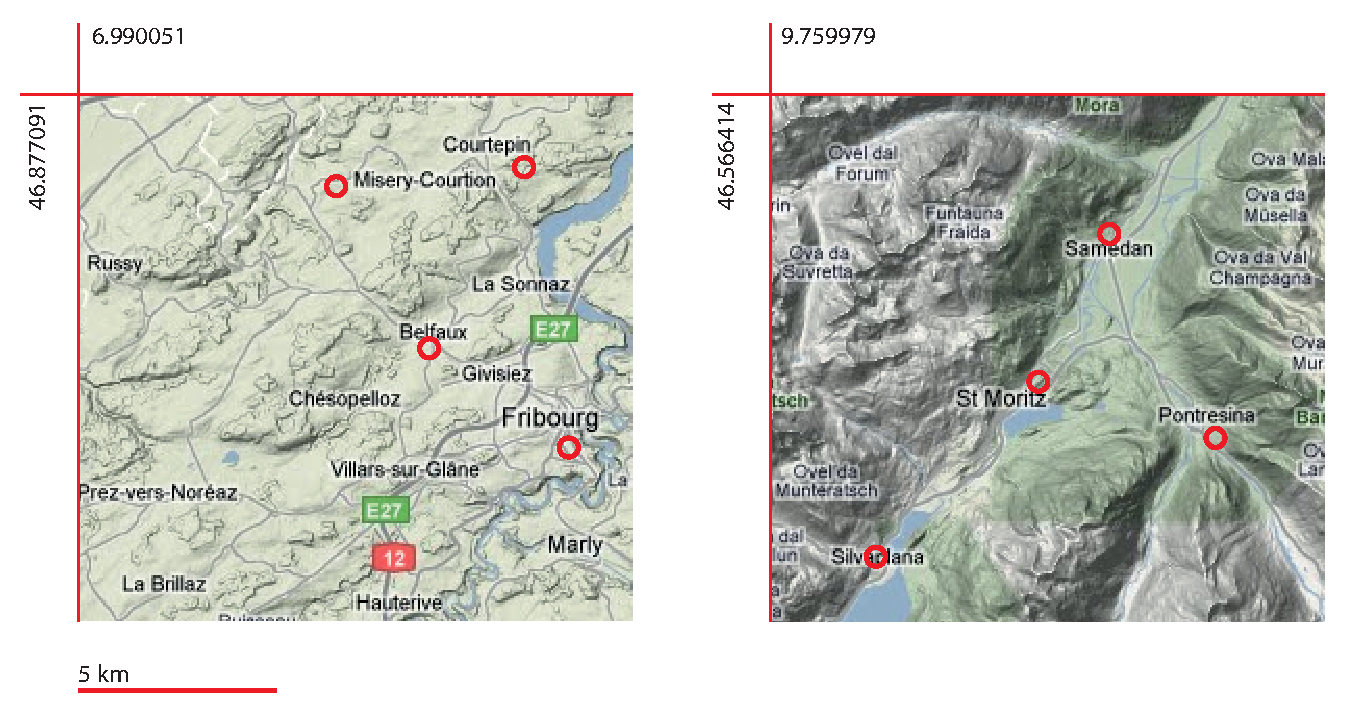
\includegraphics[width=\linewidth]{../figures/site}
	\caption{Two test sites, one mountainous one flat.}
	\label{fig:site}
\end{figure}


%=-=-=-=-=-=-=-=-=-=-=-=-=-=-=-=-=-=-=-=-=-=-=-=-=-=-=-=-=-=-=-=-=-=
\section{Expected Results}
%=-=-=-=-=-=-=-=-=-=-=-=-=-=-=-=-=-=-=-=-=-=-=-=-=-=-=-=-=-=-=-=-=-=

%(What are the answers to the above questions that you expect to find before starting your research?)

We expect to find that the smaller roads correspond more closely to results generated by the active walker model, while larger cantonal roads, being further removed from their trail origins, should correspond less with model results. We further expect increasingly mountainous terrain to tightly constrain possible routes: we expect closer correlation between road systems and generated model results in mountainous regions than in the lowlands, since there are less possibilities for taking a route with low associated energy cost.



%=-=-=-=-=-=-=-=-=-=-=-=-=-=-=-=-=-=-=-=-=-=-=-=-=-=-=-=-=-=-=-=-=-=
%\addcontentsline{toc}{section}{References}  % adds references section to TOC
\bibliographystyle{apalike2}
\bibliography{references}


\end{document}
